\subsection{HISTÓRIAS DO USUÁRIO}
\label{user_stories_sec}

Histórias do usuário é uma técnica que vem em detrimento da produção massiva de requisitos. 
Até hoje é comum achar projetos de desenvolvimento de software, com documentos de requisitos enormes. 
Com raras exceções, este não é um modelo muito produtivo. 
O grande problema é que muitas vezes gasta-se muito tempo, às vezes anos, para se criar estes documentos. 
Enquanto isso pouco ou nada de software funcional é produzido. 
Uma consequência comum desta demora, são as prioridades dos usuários mudarem, ou seja, o que foi especificado inicialmente, depois de um ano, por exemplo, já não tem o mesmo valor para os mesmos \cite{Patton2014}.

De acordo com \citeonline{cohn2004} histórias do usuário descrevem funcionalidades que serão de valor para um usuário ou comprador de um sistema de software. Histórias do usuário são compostas por três aspectos: 
\begin{itemize}
	\item Uma descrição escrita da história usada para planejamento e como lembrete;
	\item Conversações sobre a história para detalhar a mesma;
	\item Testes que trazem e documentam detalhes e que podem ser usadas para determinar quando a história está completa.
\end{itemize}

Histórias do usuário podem ser documentadas usando-se \emph{story cards}. Um exemplo é mostrado na Figura \ref{story_card}.

No \emph{story card} em questão, a parte superior é a descrição do item que é de valor para um usuário. 
A parte inferior relata testes que devem ser executados. 
Estes testes também servem para determinar se a história do usuário foi completamente implementada ou não \cite{cohn2004}.

Dentro de uma metodologia como o \emph{Scrum}, as histórias de usuário podem ser utilizadas para comporem o \emph{backlog} do produto. 
Elas são excelentes durante a fase de planejamento do \emph{sprint} \cite{Hanley2015}. 

Como as histórias do usuário são documentos mais informais, é necessário que as mesmas sejam mais detalhadas durante o processo de desenvolvimento. 
Isto pode ser feito com uma conversa entre o desenvolvedor e o \emph{product owner}. 
Pode se chegar a conclusão que a história é na verdade um "épico", ou seja, é uma história composta de outras histórias. 
Neste caso a história dever ser quebrada e suas partes enviadas para planejamento novamente \cite{cohn2004}. 

\begin{figure}[ht]
	\centering
	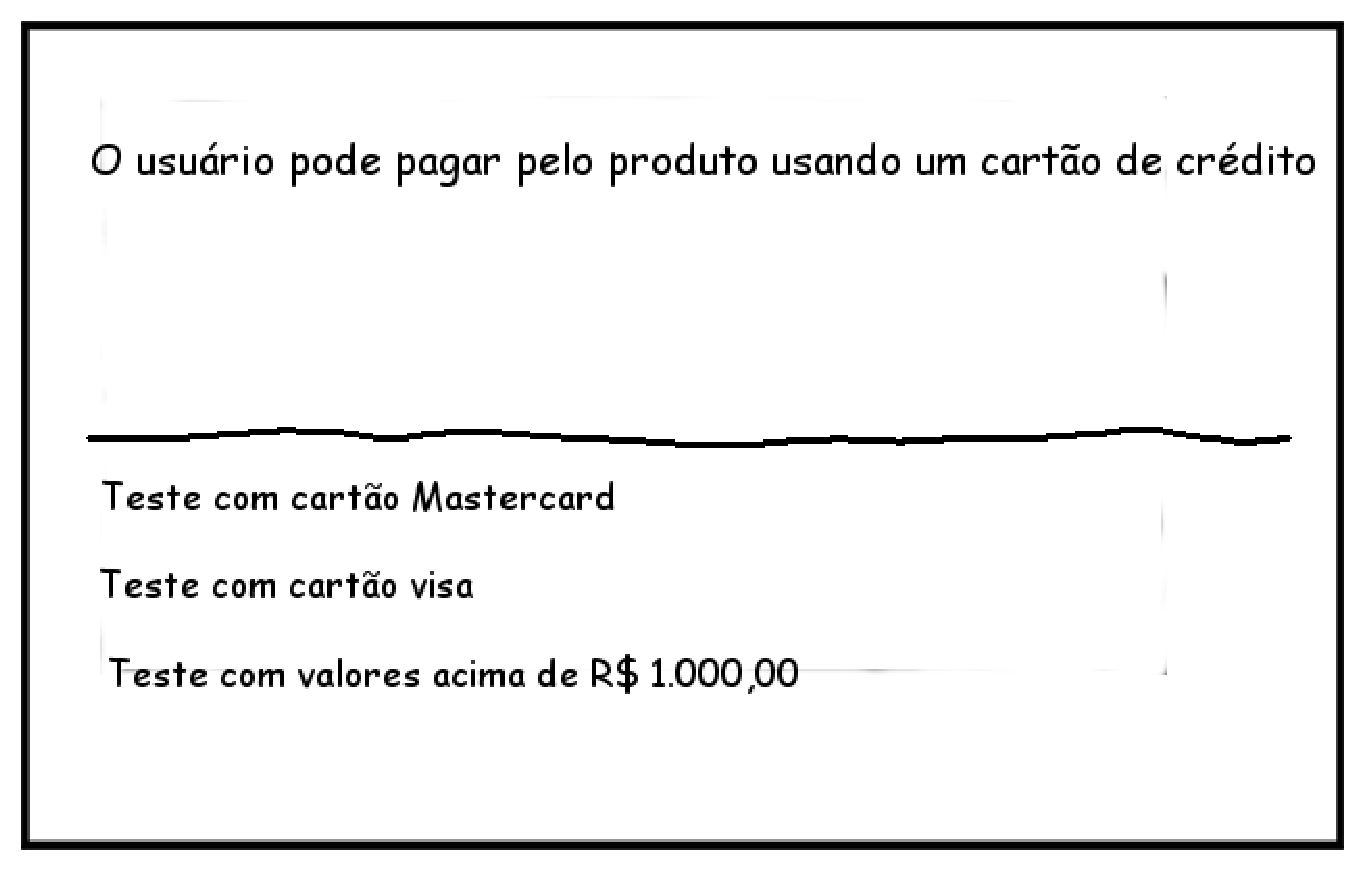
\includegraphics[width=15 cm]{figuras/story_card.eps}
	\caption{Exemplo de \emph{story card}. Fonte: (Alterado de \citeonline{cohn2004}).}
    	\label{story_card}
\end{figure}


